This chapter presents methods used to evaluate the system and the results collected evaluating the system. 

\section{Methods}

\subsection{User Survey}

The system is measured by doing user surveys on the end users. In our user survey we have coaches’ rating how much they agree with a statement on a Likert-scale. The statements compare the system against other systems in use at Alfheim today. The Likert-scale chosen is a 5 point scale from \textit{strongly disagree} to \textit{strongly agree}.\footnote{http://www.simplypsychology.org/likert-scale.html}. In short it will let each individual to note how much they disagree or agree with a particular statement.

Including to this external people not in the Tromsø IL system. This includes Ruben Yttergård Jenssen playing in the national soccer team for Norway and FC Kaiserslatern in 2. Bundesliga, and Lars Tjærnås, a previous coach and now football expert in Canal+ also writing for 100% fotball.

\section{Experiments and Results}

\subsection{Test data}

In the tests Tromsø IL academy coaches has been evaluating the system. In the evaluation phase the database had been populated with data from Tromsø IL and Strømsgodset Toppfotball matches. Only attacks from these two teams have been used in the evaluating process. A total of 34 attacks have been captured for Strømsgodset over 5 matches. For Tromsø a total of 42 attacks have been captured over 9 matches. Figure \ref{fig:matches_regged} lists all matches. Some matches include data from other teams than Tromsø and Strømsgodset. They have not been taken into consideration in the evaluating process.

\begin{figure}[ht!]
\centering
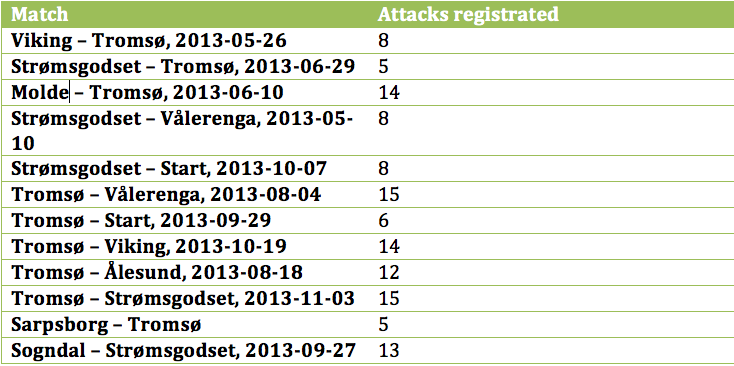
\includegraphics[width=1\textwidth]{images/general/matched_regged.png}
\caption{Matches that have been captured and persisted into the database}
\label{fig:matches_regged}
\end{figure}

\subsection{Results}

Insert figure of user servey result

\section{Limitations}

\subsection{Input}
As the input is manual the current biggest limitations is humans. There is minimal quality checking of the data. You have to trust the operator that is capturing match data. The input is to some degree subjective for some data like identifying breakthroughs. In some situations one operator may say that it was a breakthrough and another wouldn’t agree.

